\documentclass[a4paper,12pt]{article}

\usepackage[margin=1in]{geometry}
\usepackage{amsmath,amssymb,amsfonts,amsthm}
\usepackage{mathtools}
\usepackage{tikz}
\setcounter{MaxMatrixCols}{20}
\usepackage{bm}
\usepackage{enumitem}
\usepackage{graphicx}
\usepackage{hyperref}
\usepackage{xcolor}
\usepackage{ascmac}
\usepackage[normalem]{ulem}

\setlength{\parindent}{0pt}
\setlength{\parskip}{0.8em}

\newcommand{\dd}{\,d}
\newcommand{\R}{\mathbb{R}}
\newcommand{\add}[1]{\textcolor{blue}{#1}}
\newcommand{\del}[1]{\textcolor{red}{\sout{#1}}}

\begin{document}
% \pagestyle{plain}

\begin{center}
\begin{large}
\textbf{Homework \#5 ---  MATH 463 (Mathematical Biology)\\
Self-study problems with solutions}
\end{large}\\
\end{center}

\begin{screen}
\begin{itemize}
\item Due 11/23/2026, \textbf{Monday}, 11:59pm. Submit on Gradescope.
\end{itemize}
\end{screen}

As in the previous homework assignments, I generated this by Claude Opus 5.5, by feeding my section 9, 10, and 11 lecture notes, and then checked and modified it carefully.

Problems 1 and 2 are on section 9 (network biology), covering the part that HW4 did not, that is, pp.~9--25 of those lecture notes. Problems 3--6 are on section 10 (mathematical ecology). Problems 7--9 are on section 11 (evolutionary game theory), up to and including direct reciprocity, that is, pp.~1--20 of those lecture notes.

Every problem here can be done by hand (or at least most problems). There is no coding in this homework, because it is meant as preparation for the midterm exam.

\begin{enumerate}

\item Self-study \textbf{at least three} of the following problems, including at least one from each of the three topics (networks, ecology, evolutionary games). Submit your work, such as hand-written notes or typed notes, as a single pdf (yes, pdf).
\begin{itemize}
\item For other instructions and overarching goals of HW, see the face page of HW1.
\end{itemize}

\end{enumerate}

\newpage

\section*{Problems}

\subsection*{Problem 1. Your friends have more friends than you do}

In an undirected network, the degree $k_i$ of node $i$ is the number of neighbors that node $i$ has, $p(k)$ is the fraction of the nodes whose degree is $k$, and we write
\[ \left\langle k \right\rangle = \sum_{k=0}^{N-1} k\,p(k) = \frac{1}{N}\sum_{i=1}^{N} k_i,
\qquad
\left\langle k^2 \right\rangle = \sum_{k=0}^{N-1} k^2 p(k) = \frac{1}{N}\sum_{i=1}^{N} k_i^2 \]
for the mean degree and the mean of the squared degree. Consider the network with $N=7$ nodes given by
\[ V = \left\{ 1,2,3,4,5,6,7 \right\},
\qquad
E = \Big\{ (1,2),\ (1,3),\ (1,4),\ (1,5),\ (2,3),\ (5,6),\ (6,7) \Big\} . \]

\begin{enumerate}[label=(\alph*)]
\item Draw this network. Compute $k_1,\ldots,k_7$, write down $p(k)$, and compute $\left\langle k \right\rangle$.

\item Now we sample a person not at random but through a friendship: pick one of the $\left| E \right|$ edges uniformly at random, and then pick one of its two endpoints uniformly at random. Show that this procedure returns node $i$ with probability
\[ \Pr(\text{node } i) = \frac{k_i}{2\left| E \right|} = \frac{k_i}{N\left\langle k \right\rangle} , \]
and say in one sentence what is wrong with the naive guess $\frac{1}{N}$.

\item Show that the expected degree of the node sampled in (b) is
\[ \left\langle k \right\rangle_{\text{neighbor}} = \frac{\left\langle k^2 \right\rangle}{\left\langle k \right\rangle} . \]
Compute $\left\langle k^2 \right\rangle$ and $\left\langle k \right\rangle_{\text{neighbor}}$ for the network above, and compare the latter with $\left\langle k \right\rangle$ from (a).

\item Show that
\[ \frac{\left\langle k^2 \right\rangle}{\left\langle k \right\rangle} \geq \left\langle k \right\rangle \]
in every network, and that equality holds if and only if all the nodes have the same degree. (Hint: variance.) This is the friendship paradox: on average, your friends have more friends than you do.

\item For the Erd\H{o}s--R\'enyi random graph, in which each of the $\frac{N(N-1)}{2}$ node pairs is connected independently with probability $q$, the degree of a node is a binomial random variable with
\[ \left\langle k \right\rangle = (N-1)q,
\qquad
\left\langle k^2 \right\rangle - \left\langle k \right\rangle^2 = (N-1)q(1-q) . \]
Show that
\[ \left\langle k \right\rangle_{\text{neighbor}} = \left\langle k \right\rangle + 1 - q , \]
so that for a large and sparse network your friend has about one more friend than you do.

\item Suppose you can vaccinate only $n$ people in a population of $N \gg n$ individuals, and that you do not know the contact network. Someone proposes the following: choose $n$ people uniformly at random, ask each of them to name one friend, and vaccinate the friends instead of the people you chose. Using (b)--(d), explain in a few sentences why this is better than vaccinating the $n$ randomly chosen people themselves. No computation is needed.
\end{enumerate}

\subsection*{Problem 2. Heavy tails, hubs, and the epidemic threshold}

Many empirical networks have a heavy-tailed degree distribution. The standard idealization is the power law
\[ p(k) = C k^{-\gamma} \qquad (k \geq k_{\min}), \]
where we treat the degree $k$ as a continuous variable so that sums over $k$ become integrals, and $k_{\min}>0$ is the smallest degree present.

We will also use the following result from the SIR model on networks (section 9; recall the SIS model of section 4). If each infected node infects each of its susceptible neighbors at rate $\beta$ and recovers at rate $\mu$, then a large outbreak is possible only if $\beta>\beta_{\text{c}}$, where
\[ \beta_{\text{c}} = \frac{\left\langle k \right\rangle}{\left\langle k^2 \right\rangle - \left\langle k \right\rangle}\, \mu . \]

\begin{enumerate}[label=(\alph*)]
\item Determine $C$ from $\int_{k_{\min}}^{\infty} p(k) \dd k = 1$. For which $\gamma$ does the integral converge?

\item The complementary cumulative distribution is defined by $\bar{F}(k) = \int_{k}^{\infty} p(k')\dd k'$, that is, the fraction of nodes whose degree exceeds $k$. Show that
\[ \bar{F}(k) = \left( \frac{k}{k_{\min}} \right)^{-(\gamma-1)} . \]
Then show that both $\ln p(k)$ and $\ln \bar{F}(k)$ are linear functions of $\ln k$, and give the slope of each.

\item Show that
\[ \left\langle k \right\rangle = \frac{\gamma-1}{\gamma-2} k_{\min} \quad (\gamma>2),
\qquad
\left\langle k^2 \right\rangle = \frac{\gamma-1}{\gamma-3} k_{\min}^2 \quad (\gamma>3) . \]
Show also that for $2<\gamma\leq 3$ the integral defining $\left\langle k^2 \right\rangle$ diverges while the one defining $\left\langle k \right\rangle$ still converges.

\item What does the result of (c) imply about the epidemic threshold $\beta_{\text{c}}$ of a heavy-tailed network with $2<\gamma<3$, which is the range that most empirical networks fall in? What does your answer mean for a disease that spreads on such a network?
\end{enumerate}

\subsection*{Problem 3. Does complexity make an ecosystem stable?}

Let $S$ species coexist at an equilibrium $\bm{x}^* = \left( x_1^*,\ldots,x_S^* \right)^{\top}$ of some population dynamics $\frac{\dd \bm{x}}{\dd t} = f(\bm{x})$, and let $\bm{z} = \bm{x}-\bm{x}^*$ be a deviation from it. To first order, $\frac{\dd \bm{z}}{\dd t} = M \bm{z}$, where the $S\times S$ matrix $M$ is the Jacobian of $f$ at $\bm{x}^*$, called the community matrix (it was introduced in class); $M_{ij}$ measures the effect of species $j$ on the growth of species $i$ near the equilibrium.

May (1972) asked what happens if $M$ is built at random:
\begin{itemize}
\item $M_{ii}=-1$ for every $i$ (each species regulates itself);
\item each off-diagonal entry is nonzero with probability $C$ (called the connectance), independently;
\item a nonzero off-diagonal entry is drawn from a distribution with mean $0$ and variance $\sigma^2$.
\end{itemize}
For large $S$, the eigenvalues of such an $M$ fill a disk in the complex plane centered at $(-1,0)$ with radius $\sigma\sqrt{SC}$. Recall that the equilibrium is locally stable if and only if every eigenvalue of $M$ has a negative real part.

\begin{enumerate}[label=(\alph*)]
\item Using the disk, show that the community is stable (almost surely, for large $S$) if and only if
\[ \sigma\sqrt{SC} < 1,
\qquad\text{that is,}\qquad
S < \frac{1}{\sigma^2 C} . \]
Compute the largest number of species that can coexist stably when $\sigma=0.1$ and $C=0.5$, and then when $\sigma$ is doubled to $0.2$ with $C$ unchanged.

\item State in one sentence why this result was a surprise to ecologists.

\item May's matrix ignores the fact that a pair of species interacts in a particular way. Take $S=2$ and
\[ M = \begin{pmatrix} -1 & a\\ b & -1 \end{pmatrix} . \]
Show that the eigenvalues of $M$ are $-1 \pm \sqrt{ab}$. Then determine the stability of the equilibrium in each of the following three cases, and in each case say for which values of $a$ and $b$ the equilibrium is stable:
	\begin{itemize}
	\item predator--prey, $a>0$ and $b<0$ (species 2 helps species 1, species 1 harms species 2);
	\item mutualism, $a>0$ and $b>0$;
	\item competition, $a<0$ and $b<0$.
	\end{itemize}

\item Allesina and Tang (2012) did the large-$S$ version of (c), and found that the eigenvalue cloud is no longer a disk: it is an ellipse that is stretched vertically (along the imaginary axis) for predator--prey interactions and stretched horizontally (along the real axis) for mutualism and competition. Using the eigenvalues that you computed in (c), explain in two or three sentences why that is exactly what you would expect, and which type of food web can therefore afford to be the most complex.
\end{enumerate}

\subsection*{Problem 4. Rock--paper--scissors in a well-mixed population}

Three types of individual, R, S, and P, cyclically dominate one another: R beats S, S beats P, and P beats R. When two individuals of different types meet, the dominant one converts the other into its own type,
\[ \text{R}+\text{S} \to \text{R}+\text{R},
\qquad
\text{S}+\text{P} \to \text{S}+\text{S},
\qquad
\text{P}+\text{R} \to \text{P}+\text{P} . \]
Let $r$, $s$, and $p$ be the fractions of the three types, with $r+s+p=1$. In a well-mixed population, mass action gives the cyclic Lotka--Volterra model
\[
\frac{\dd r}{\dd t} = r\left( s-p \right),
\qquad
\frac{\dd s}{\dd t} = s\left( p-r \right),
\qquad
\frac{\dd p}{\dd t} = p\left( r-s \right).
\]

\begin{enumerate}[label=(\alph*)]
\item Show that $\frac{\dd}{\dd t}\left( r+s+p \right)=0$, so that a trajectory that starts on the simplex $r+s+p=1$ stays on it. What does this mean biologically?

\item Find all the equilibria of the system on the simplex. (Do not forget to check whether there is an equilibrium in the interior of an edge of the simplex, that is, with exactly one of $r,s,p$ equal to zero.)

\item Show that $H \equiv rsp$ does not change in time. Explain why this implies that every trajectory in the interior of the simplex is a closed orbit, so that the interior equilibrium is neither attracting nor repelling.

\end{enumerate}

\subsection*{Problem 5. How to read the triangle}

Problem 4, and Figure~4 of the section~10 lecture notes, drew the state of a three-type population as a point inside a triangle. This problem is about how to read that picture. The same picture is used for the three genotypes AA, Aa, and aa in population genetics, and for any model with three types or three strategies, so it is worth being fluent with it.

The set of possible states is
\[ \Delta = \left\{ \left( r,s,p \right) \in \R^3 \ : \ r \geq 0, \ s \geq 0, \ p \geq 0, \ r+s+p=1 \right\} . \]
This set is called the 2-simplex. We draw it as follows. Fix an equilateral triangle whose corners are $V_{\text{R}}$, $V_{\text{S}}$, and $V_{\text{P}}$, and draw the state $\left( r,s,p \right)$ at the point
\[ X = r V_{\text{R}} + s V_{\text{S}} + p V_{\text{P}} \]
of the plane. You should regard $V_{\text{R}}$, $V_{\text{S}}$, and $V_{\text{P}}$ as two-dimensional vectors.
Because $r,s,p \geq 0$ and $r+s+p=1$, the point $X$ is a weighted average of the three corners and therefore lies inside the triangle, and the three weights $\left( r,s,p \right)$ are called the barycentric coordinates of $X$. In population genetics, the same picture is known as a de Finetti diagram.

Figure~\ref{fig:simplex} is used throughout this problem.

\begin{figure}[htbp]
\begin{center}
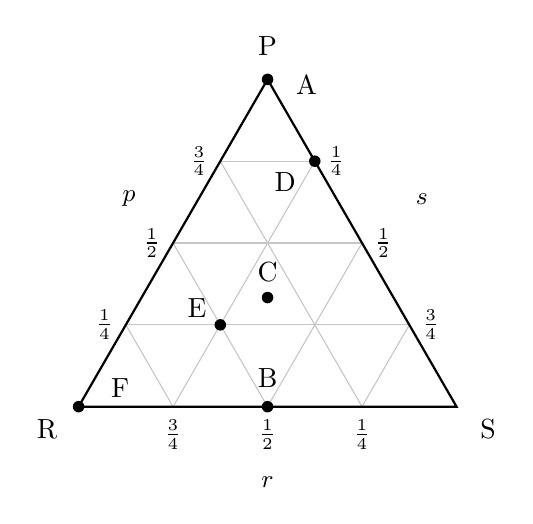
\begin{tikzpicture}[scale=0.8]
% --- grid lines: p = const (horizontal), r = const, s = const ---
\draw[gray!45] (0.75,1.299) -- (5.25,1.299);
\draw[gray!45] (1.50,2.598) -- (4.50,2.598);
\draw[gray!45] (2.25,3.897) -- (3.75,3.897);
\draw[gray!45] (4.50,0) -- (2.25,3.897);
\draw[gray!45] (3.00,0) -- (1.50,2.598);
\draw[gray!45] (1.50,0) -- (0.75,1.299);
\draw[gray!45] (1.50,0) -- (3.75,3.897);
\draw[gray!45] (3.00,0) -- (4.50,2.598);
\draw[gray!45] (4.50,0) -- (5.25,1.299);
% --- triangle ---
\draw[thick] (0,0) -- (6,0) -- (3,5.196) -- cycle;
% --- corner labels ---
\node at (-0.5,-0.35) {R};
\node at (6.5,-0.35) {S};
\node at (3,5.72) {P};
% --- tick labels: r on the lower side, p on the left side, s on the right side ---
\node[below,font=\small] at (1.50,-0.06) {$\frac{3}{4}$};
\node[below,font=\small] at (3.00,-0.06) {$\frac{1}{2}$};
\node[below,font=\small] at (4.50,-0.06) {$\frac{1}{4}$};
\node[below,font=\small] at (3.00,-0.95) {$r$};
\node[left,font=\small] at (0.70,1.299) {$\frac{1}{4}$};
\node[left,font=\small] at (1.45,2.598) {$\frac{1}{2}$};
\node[left,font=\small] at (2.20,3.897) {$\frac{3}{4}$};
\node[font=\small] at (0.80,3.30) {$p$};
\node[right,font=\small] at (3.80,3.897) {$\frac{1}{4}$};
\node[right,font=\small] at (4.55,2.598) {$\frac{1}{2}$};
\node[right,font=\small] at (5.30,1.299) {$\frac{3}{4}$};
\node[font=\small] at (5.45,3.30) {$s$};
% --- the six marked points ---
\fill (3.00,5.196) circle (2.6pt);  \node at (3.62,5.10) {A};
\fill (3.00,0)     circle (2.6pt);  \node at (3.00,0.45) {B};
\fill (3.00,1.732) circle (2.6pt);  \node at (3.00,2.13) {C};
\fill (3.75,3.897) circle (2.6pt);  \node at (3.28,3.56) {D};
\fill (2.25,1.299) circle (2.6pt);  \node at (1.88,1.56) {E};
\fill (0,0)        circle (2.6pt);  \node at (0.66,0.30) {F};
\end{tikzpicture}
\hfill
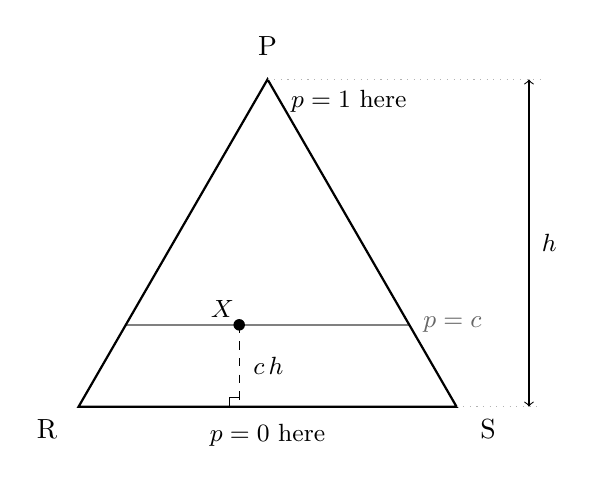
\begin{tikzpicture}[scale=0.8]
% --- the line p = c, and the triangle ---
\draw[gray,thick] (0.75,1.299) -- (5.25,1.299);
\draw[thick] (0,0) -- (6,0) -- (3,5.196) -- cycle;
\node at (-0.5,-0.35) {R};
\node at (6.5,-0.35) {S};
\node at (3,5.72) {P};
% --- the point X = (0.45, 0.30, 0.25), that is, p = c = 1/4 ---
\fill (2.55,1.299) circle (2.6pt);
\node[above left,font=\small,inner sep=1pt] at (2.52,1.36) {$X$};
\draw[dashed] (2.55,1.299) -- (2.55,0);
\draw (2.40,0) -- (2.40,0.15) -- (2.55,0.15);          % right angle at the foot
\node[right,font=\small] at (2.62,0.65) {$c\,h$};
\node[right,font=\small,gray!80!black] at (5.32,1.299) {$p=c$};
% --- what p is on the side RS and at the corner P ---
\node[below,font=\small] at (3.00,-0.12) {$p=0$ here};
\node[right,font=\small] at (3.22,4.85) {$p=1$ here};
% --- the height of the triangle ---
\draw[gray!60,dotted] (6,0) -- (7.35,0);
\draw[gray!60,dotted] (3,5.196) -- (7.35,5.196);
\draw[<->] (7.15,0) -- (7.15,5.196);
\node[right,font=\small] at (7.20,2.60) {$h$};
\end{tikzpicture}
\caption{The simplex $\Delta$, drawn as a triangle whose corners are the three pure states R, S, and P.
Left: the six points A--F of Problem 5(d). The thin lines are the lines along which one of the three fractions is $\frac{1}{4}$, $\frac{1}{2}$, or $\frac{3}{4}$; the tick labels on the lower, left, and right sides belong to $r$, $p$, and $s$, respectively.
Right: the rule of Problem 5(e), drawn for $p$. The gray line consists of all the states whose $p$ equals a given value $c$. It is parallel to the side RS, which is the side \underline{opposite} the P corner, and it lies at distance $c\,h$ from that side, where $h$ is the height of the triangle. So $p$ grows in proportion to the distance from the side RS, from $p=0$ on that side to $p=1$ at the opposite corner P. The same holds for $r$ with the side SP, and for $s$ with the side RP.}
\label{fig:simplex}
\end{center}
\end{figure}

\begin{enumerate}[label=(\alph*)]
\item Explain why $\Delta$, whose elements are triples of numbers, is a two-dimensional object, which is what makes a faithful drawing of it in the plane possible in the first place.

\item Put $V_{\text{R}}=\left( 0,0 \right)$, $V_{\text{S}}=\left( 1,0 \right)$, and $V_{\text{P}}=\left( \frac{1}{2},\frac{\sqrt{3}}{2} \right)$, so that the triangle has side $1$ and height $h=\frac{\sqrt{3}}{2}$. Compute the Cartesian coordinates $\left( x,y \right)$ of the drawn point $X$ in terms of $\left( r,s,p \right)$. Where in the triangle is the state $\left( \frac13,\frac13,\frac13 \right)$ drawn?

\item Invert the formulas of (b), that is, recover $\left( r,s,p \right)$ from the coordinates $\left( x,y \right)$ of a point of the triangle. Check that your three expressions add up to $1$.

\item For each of the six points A--F marked in Figure~\ref{fig:simplex} (left), read off $\left( r,s,p \right)$ and say how many of the three types are present. Which of the six points is the interior equilibrium of Problem 4?

\item Show that the states with $p$ equal to a fixed value $c \in \left[ 0,1 \right]$ are drawn on a straight line segment that is parallel to the side $V_{\text{R}}V_{\text{S}}$ and at distance $c\,h$ from it, where $h$ is the height of the triangle. Figure~\ref{fig:simplex} (right) draws this statement. Permuting the roles of the three coordinates then gives the general rule: the distance from a point $X$ to a side of the triangle, divided by $h$, is the fraction of the type that sits at the corner opposite that side.

Which side of the triangle does a trajectory approach when type R becomes rare?

\item Show that in the dynamics of Problem 4 each of the three sides of the triangle is invariant, that is, a type that is absent at $t=0$ is absent forever, and that on the side $p=0$ the system reduces to the logistic equation $\frac{\dd r}{\dd t} = r\left( 1-r \right)$.

What does a side of the triangle mean biologically, and what does a corner mean?

\item In Figure~4 of the section~10 lecture notes, the middle triangle (a finite well-mixed population) ends with a dot at a corner, whereas the right triangle (the same number of individuals on a square lattice) keeps winding around the center of the triangle. Say in one or two sentences each what these two pictures tell you about the fate of the population.
\end{enumerate}

\subsection*{Problem 6. Critical slowing down before a tipping point}

A harvested population obeys
\[ \frac{\dd x}{\dd t} = f(x) = x\left( 1-x \right) - h, \]
where $x \geq 0$ is the population density and $h \geq 0$ is the constant harvesting rate.

We will use the following fact about a population that is being watched near a stable equilibrium $x^*$ while small random disturbances (``noise'') keep pushing it around. Write $\lambda = f'(x^*) < 0$ for the recovery rate. Then, in the long run, the variance of the measured $x$ is
\[ V = \frac{\sigma^2}{2\left| \lambda \right|} , \]
where $\sigma^2$ measures the strength of the noise and does not change as $h$ is varied.

\begin{enumerate}[label=(\alph*)]
\item Find the two equilibria of the system for $0<h<\frac{1}{4}$, and determine the stability of each. What happens to them at $h=\frac{1}{4}$, and what happens to the population for $h>\frac{1}{4}$? Which bifurcation is this?

\item Show that the recovery rate at the stable equilibrium $x_+$ is
\[ \lambda = -\sqrt{1-4h} , \]
so that $\lambda \to 0^-$ as $h \to \frac{1}{4}^-$. This is critical slowing down.

Compute $\lambda$ and the return time $\frac{1}{\left| \lambda \right|}$ (the time it takes a small deviation to shrink by the factor $\text{e}$) for $h=0.24$ and for $h=0.2475$. You may use $\sqrt{0.04}=0.2$ and $\sqrt{0.01}=0.1$.

\item Compute the ratio of the variance $V$ at $h=0.2475$ to the variance at $h=0.24$. Which of the two populations has the noisier time series, the one that is harvested closer to the critical rate or the other one?
\end{enumerate}

\subsection*{Problem 7. Evolutionarily stable strategies and the hawk--dove game}

In a symmetric two-player game, let $u(x,y)$ be the payoff to a player using strategy $x$ against an opponent using strategy $y$. Strategies may be mixed, that is, probability distributions over the pure strategies.
\begin{itemize}
\item $x$ is a Nash equilibrium if $u(x,x) \geq u(y,x)$ for every $y$.
\item $x$ is a strict Nash equilibrium if $u(x,x) > u(y,x)$ for every $y \neq x$.
\item $x$ is an evolutionarily stable strategy (ESS) if and only if, for every $y \neq x$,
	\begin{enumerate}[label=(\roman*)]
	\item $u(x,x) \geq u(y,x)$, and
	\item if $u(x,x) = u(y,x)$, then $u(x,y)>u(y,y)$.
	\end{enumerate}
\end{itemize}
The second condition of the ESS is what makes the definition evolutionary: it says that, when the mutant does equally well against the resident as the resident does against itself, the tie has to be broken in the resident's favor in the rare encounters between two mutants.

Two animals contest a resource worth $V>0$. A Hawk (H) escalates and fights; a Dove (D) displays and retreats. Two Hawks fight, and the cost $c>0$ of the fight is shared, so each gets $\frac{V-c}{2}$ on average. A Hawk facing a Dove takes the whole resource. Two Doves share the resource. Thus, with the rows being the focal player's strategy and the columns the opponent's,
\[ A = \begin{pmatrix} \frac{V-c}{2} & V \\[2pt] 0 & \frac{V}{2} \end{pmatrix} . \]

\begin{enumerate}[label=(\alph*)]
\item Show that every strict Nash equilibrium is an ESS.

\item Explain in one or two sentences why a Nash equilibrium that is not strict need not be an ESS.

\item Cheap fights, $V>c$. Show that H is a strict Nash equilibrium, and hence an ESS, and that D is not a Nash equilibrium. What does the model predict about the behavior of the animals?

\item Costly fights, $V<c$. Show that neither H nor D is a Nash equilibrium.

\end{enumerate}

\subsection*{Problem 8. Replicator dynamics}

In a large, well-mixed population, let $x_i$ be the fraction of the individuals using strategy $s_i$, let $u(s_i,x)$ be the expected payoff of an $s_i$-player against a uniformly randomly chosen member of the population, and let $u(x,x)=\sum_j x_j u(s_j,x)$ be the mean payoff in the population. The replicator equation is
\[ \frac{\dd x_i}{\dd t} = x_i\left[ u(s_i,x) - u(x,x) \right] . \]

\begin{enumerate}[label=(\alph*)]
\item Say in one or two sentences what this equation means, in words, and why the right-hand side has a factor $x_i$ in front.

\item Consider two strategies, $1$ and $2$, with payoff matrix
\[ A = \begin{pmatrix} a & b\\ c & d \end{pmatrix} \]
(so that $a=u(s_1,s_1)$, $b=u(s_1,s_2)$, and so on), and let $x$ be the fraction of the population using strategy $1$, so that $1-x$ use strategy $2$. Show that
\[ \frac{\dd x}{\dd t} = x(1-x)\Big[ (a-c)x + (b-d)(1-x) \Big] . \]

\item The prisoner's dilemma with $R=3$, $S=0$, $T=5$, $P=1$, that is,
\[ A = \begin{pmatrix} 3 & 0\\ 5 & 1 \end{pmatrix} , \]
where strategy $1$ is to cooperate (C) and strategy $2$ is to defect (D). Show that
\[ \frac{\dd x}{\dd t} = -x(1-x)(1+x) . \]
Find all the equilibria in $[0,1]$, determine their stability, draw the phase portrait on $[0,1]$, and state the conclusion about cooperation.

\item The coordination game $R=5$, $S=0$, $T=0$, $P=3$, that is,
\[ A = \begin{pmatrix} 5 & 0\\ 0 & 3 \end{pmatrix} . \]
Show that $\frac{\dd x}{\dd t} = x(1-x)(8x-3)$, find all the equilibria in $[0,1]$ and their stability, and draw the phase portrait. What does the interior equilibrium mean for a population that is trying to switch from the all-D state to the all-C state?

\item The hawk--dove game of Problem 7 with resource value $V=2$ and fight cost $4$, that is,
\[ A = \begin{pmatrix} -1 & 2\\ 0 & 1 \end{pmatrix} , \]
where strategy $1$ is H. Show that $\frac{\dd x}{\dd t} = x(1-x)(1-2x)$, and show that the interior equilibrium is asymptotically stable.

\end{enumerate}

\subsection*{Problem 9. Direct reciprocity: the repeated prisoner's dilemma}

Two players play the prisoner's dilemma game with payoff matrix
\[ A = \begin{pmatrix} R & S\\ T & P \end{pmatrix} = \begin{pmatrix} 3 & 0\\ 5 & 1 \end{pmatrix} \]
(rows and columns ordered C, D) repeatedly. After each round, another round is played with probability $w$, where $0<w<1$, and the game ends with probability $1-w$. A player's score is the sum of the payoffs over all the rounds that are played. Consider three strategies:
\begin{itemize}
\item ALLC: cooperate in every round;
\item ALLD: defect in every round;
\item TFT (tit-for-tat): cooperate in the first round, and from then on do whatever the opponent did in the previous round.
\end{itemize}

\begin{enumerate}[label=(\alph*)]
\item Show that the expected number of rounds played is $\frac{1}{1-w}$.

\item What is the largest expected score that a player could conceivably obtain, and against which opponent?

\item Compute the expected score of each of the two players in each of the following five pairings: TFT versus TFT, TFT versus ALLD, TFT versus ALLC, ALLD versus ALLC, and ALLD versus ALLD.

\item Consider a large population in which almost everybody plays TFT, and a few mutants play ALLD. Using (b), show that TFT resists the invasion, that is, that a TFT player earns strictly more than an ALLD mutant, if and only if
\[ w > \frac{T-R}{T-P} = \frac{1}{2} . \]
Interpret the condition in words: what has to be true about the relationship for reciprocity to pay?

\item Now let the mutants play ALLC instead. Compute $u(\text{TFT},\text{TFT})$, $u(\text{ALLC},\text{TFT})$, $u(\text{TFT},\text{ALLC})$, and $u(\text{ALLC},\text{ALLC})$, and use the ESS conditions of Problem 7 to show that TFT is not an ESS, no matter how large $w$ is. What is then likely to happen to a population of TFT players over a long time, if ALLD mutants also appear occasionally?

\end{enumerate}

\newpage

\section*{Solutions}

\subsection*{Solution to Problem 1}

\begin{enumerate}[label=(\alph*)]
\item Nodes $1$, $2$, and $3$ form a triangle; node $4$ hangs off node $1$; and $1-5-6-7$ is a path:
\begin{center}
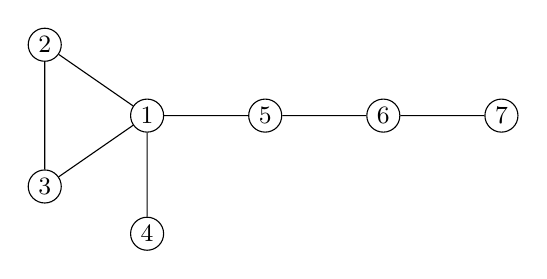
\begin{tikzpicture}[scale=1.0,every node/.style={circle,draw,inner sep=1.6pt,font=\small}]
\node (n2) at (-1.3,0.9) {2};
\node (n3) at (-1.3,-0.9) {3};
\node (n1) at (0,0) {1};
\node (n4) at (0,-1.5) {4};
\node (n5) at (1.5,0) {5};
\node (n6) at (3.0,0) {6};
\node (n7) at (4.5,0) {7};
\draw (n1)--(n2) (n1)--(n3) (n2)--(n3) (n1)--(n4) (n1)--(n5) (n5)--(n6) (n6)--(n7);
\end{tikzpicture}
\end{center}
Counting the neighbors of each node,
\[ k_1=4, \quad k_2=2, \quad k_3=2, \quad k_4=1, \quad k_5=2, \quad k_6=2, \quad k_7=1 . \]
Two nodes have degree $1$, four have degree $2$, and one has degree $4$, so
\[ p(1)=\frac{2}{7}, \qquad p(2)=\frac{4}{7}, \qquad p(4)=\frac{1}{7}, \qquad p(k)=0 \ \text{ otherwise} , \]
and
\[ \left\langle k \right\rangle = \frac{1}{7}\left( 4+2+2+1+2+2+1 \right) = \frac{14}{7} = 2 . \]
(Check: $\sum_i k_i = 14 = 2\left| E \right|$ with $\left| E \right|=7$.)

\item Each edge is chosen with probability $\frac{1}{\left| E \right|}$ and then each of its two endpoints with probability $\frac{1}{2}$, so each (edge, endpoint) pair is obtained with probability $\frac{1}{2\left| E \right|}$. Node $i$ is obtained from exactly those pairs whose edge is one of the $k_i$ edges attached to node $i$, so
\[ \Pr(\text{node } i) = \frac{k_i}{2\left| E \right|} = \frac{k_i}{\sum_{j=1}^{N}k_j} = \frac{k_i}{N\left\langle k \right\rangle} , \]
where we used $\sum_j k_j = 2\left| E \right|$.

The naive guess $\frac{1}{N}$ would be right if we picked a \underline{person} at random. But we are picking a \underline{friendship} at random, and a person with many friends sits at the end of many friendships, so they have many more chances of being picked. A node of degree $k_i$ is picked $k_i$ times as often as a node of degree $1$. This is a biased sample, and the bias is proportional to the degree.

\item Using (b),
\[ \left\langle k \right\rangle_{\text{neighbor}} = \sum_{i=1}^{N} k_i \Pr(\text{node } i)
= \sum_{i=1}^{N} k_i \cdot \frac{k_i}{N \left\langle k \right\rangle}
= \frac{\frac{1}{N}\sum_{i=1}^{N} k_i^2}{\left\langle k \right\rangle}
= \frac{\left\langle k^2 \right\rangle}{\left\langle k \right\rangle} . \]
For our network,
\[ \left\langle k^2 \right\rangle = \frac{1}{7}\left( 16+4+4+1+4+4+1 \right) = \frac{34}{7} , \]
so
\[ \left\langle k \right\rangle_{\text{neighbor}} = \frac{34/7}{2} = \frac{17}{7} \approx 2.43 > 2 = \left\langle k \right\rangle . \]
A person reached through a friendship has on average $2.43$ friends, whereas an average person has $2$.

\item Let $\sigma^2$ be the variance of the degree over the nodes. Then
\[ \sigma^2 = \left\langle \left( k-\left\langle k \right\rangle \right)^2 \right\rangle = \left\langle k^2 \right\rangle - \left\langle k \right\rangle^2 \geq 0 , \]
so $\left\langle k^2 \right\rangle \geq \left\langle k \right\rangle^2$, and dividing by $\left\langle k \right\rangle>0$,
\[ \frac{\left\langle k^2 \right\rangle}{\left\langle k \right\rangle} \geq \left\langle k \right\rangle . \]
Equality holds exactly when $\sigma^2=0$, that is, when every node has the same degree (a regular network). In every other network the inequality is strict.

\item Using the identity just derived,
\[ \left\langle k \right\rangle_{\text{neighbor}} = \left\langle k \right\rangle + \frac{\sigma^2}{\left\langle k \right\rangle}
= \left\langle k \right\rangle + \frac{(N-1)q(1-q)}{(N-1)q} = \left\langle k \right\rangle + 1 - q . \]
For a large sparse network, $q$ is small, so $\left\langle k \right\rangle_{\text{neighbor}} \approx \left\langle k \right\rangle+1$.

Note how modest this is: in the most homogeneous random network, the paradox amounts to exactly one extra friend, regardless of how large $\left\langle k \right\rangle$ is. Networks with heavy-tailed ($\approx$ power-law) degree distributions, where $\sigma^2$ is huge, give far more dramatic gaps; this is Problem 2.

\item By (b), a person named as a friend is sampled with probability proportional to their degree, so the named friends are on average higher-degree people than the randomly chosen ones, by (c) and (d). High-degree people matter twice over in an epidemic: they are more likely to be infected, because they have more contacts through which to catch the disease, and once infected they are more likely to pass the disease to many others. Vaccinating them therefore removes more transmission routes per vaccine.

The practical beauty of this is that it needs no knowledge of the network whatsoever: we never have to find out who the hubs are, and nobody has to report anything about themselves other than naming one friend. The strategy is known as acquaintance immunization.
\end{enumerate}

\subsection*{Solution to Problem 2}

\begin{enumerate}[label=(\alph*)]
\item
\[ \int_{k_{\min}}^{\infty} Ck^{-\gamma} \dd k
= \frac{C}{1-\gamma}\left[ k^{-\gamma+1} \right]_{k_{\min}}^{\infty}
= \frac{C}{\gamma-1}k_{\min}^{-\gamma+1} = 1 , \]
provided that $\gamma>1$, which is what makes $k^{-\gamma+1} \to 0$ as $k\to\infty$. Hence
\[ C = (\gamma-1)k_{\min}^{\gamma-1} . \]

\item The same integral with the lower limit $k$ instead of $k_{\min}$:
\[ \bar{F}(k) = \int_{k}^{\infty} C k'^{-\gamma}\dd k' = \frac{C}{\gamma-1}k^{-\gamma+1}
= k_{\min}^{\gamma-1}k^{-(\gamma-1)} = \left( \frac{k}{k_{\min}} \right)^{-(\gamma-1)} . \]
(Check: $\bar F(k_{\min})=1$, as it must be, since every node has degree at least $k_{\min}$.) Taking logarithms,
\[ \ln p(k) = \ln C - \gamma \ln k,
\qquad
\ln \bar{F}(k) = (\gamma-1)\ln k_{\min} - (\gamma-1)\ln k . \]
Both are straight lines in $\ln k$, of slope $-\gamma$ and $-(\gamma-1)$, respectively. So a power law is a straight line on a log--log plot either way, and the two slopes differ by exactly $1$.


\item With $C=(\gamma-1)k_{\min}^{\gamma-1}$,
\[ \left\langle k \right\rangle = \int_{k_{\min}}^{\infty}k\,Ck^{-\gamma}\dd k
= C\int_{k_{\min}}^{\infty}k^{-\gamma+1}\dd k
= \frac{C}{\gamma-2}k_{\min}^{-\gamma+2}
= \frac{\gamma-1}{\gamma-2}k_{\min} , \]
where the integral converges only if $-\gamma+2<0$ (because otherwise, the ``$\infty^{-\gamma+2}$ term'' does not vanish), that is, $\gamma>2$. Similarly,
\[ \left\langle k^2 \right\rangle = C\int_{k_{\min}}^{\infty}k^{-\gamma+2}\dd k
= \frac{C}{\gamma-3}k_{\min}^{-\gamma+3}
= \frac{\gamma-1}{\gamma-3}k_{\min}^2 , \]
which requires $-\gamma+3<0$, that is, $\gamma>3$.

For $2<\gamma \leq 3$ the first integral still converges, but in the second one the integrand $k^{-\gamma+2}$ decays no faster than $k^{-1}$, whose integral diverges logarithmically; hence $\left\langle k^2 \right\rangle=\infty$. In words: the mean degree is finite, but the mean of the squared degree is not, because the rare nodes of enormous degree contribute too much. Empirical networks typically have $2<\gamma<3$, that is, exactly the regime in which the second moment blows up.

\item By (c), $\left\langle k \right\rangle$ is finite for $2<\gamma<3$ but $\left\langle k^2 \right\rangle$ diverges. So,
\[ \beta_{\text{c}} = \frac{\left\langle k \right\rangle}{\left\langle k^2 \right\rangle - \left\langle k \right\rangle}\mu \longrightarrow 0. \]
A large heavy-tailed network has effectively no epidemic threshold: however small the per-contact infection rate $\beta$ is, the condition $\beta>\beta_{\text{c}}$ is met, and the disease can spread to a finite fraction of the network.

This is why the heavy-tailed distribution of the number of sexual partners reported by Liljeros et al.\, Nature (2001) is a serious matter for the control of a sexually transmitted infection: lowering $\beta$ a little, which is what most interventions do, need not push the system below the threshold, because there is essentially no threshold to get below. The accompanying good news is that targeting the hubs is very effective, as in Problem 1(f).

The mechanism behind the vanishing threshold is the friendship paradox of Problem 1. An infected node passes the disease on \underline{along an edge}, and an edge leads to a node with probability proportional to its degree, which is exactly the biased sampling of Problem 1(b). The disease therefore reaches hubs preferentially, and a hub, once infected, has many edges along which to pass it on further.

\end{enumerate}

\subsection*{Solution to Problem 3}

\begin{enumerate}[label=(\alph*)]
\item The eigenvalue with the largest real part is the rightmost point of the disk, which lies at $-1 + \sigma\sqrt{SC}$ on the real axis. All the eigenvalues have a negative real part if and only if this rightmost point is negative, that is,
\[ -1+\sigma\sqrt{SC} < 0
\quad\Longleftrightarrow\quad
\sigma\sqrt{SC}<1
\quad\Longleftrightarrow\quad
\sigma^2 SC<1
\quad\Longleftrightarrow\quad
S < \frac{1}{\sigma^2 C} . \]
With $\sigma=0.1$ and $C=0.5$,
\[ S < \frac{1}{(0.1)^2 \times 0.5} = \frac{1}{0.005} = 200 . \]
With $\sigma=0.2$ and the same $C$,
\[ S < \frac{1}{(0.2)^2 \times 0.5} = \frac{1}{0.02} = 50 . \]

\item Because it says the opposite of what ecologists had believed. The older intuition (explained in class) was that a richer community, with more species and more interactions, is more robust. May's calculation says that each of the three ways of being more complex, namely more species $S$, denser interactions $C$, and stronger interactions $\sigma$, makes stability \underline{less} likely, and that the three trade off against one another through the single combination $\sigma\sqrt{SC}$. The puzzle it creates is then: why do real, species-rich ecosystems persist at all?

\item The characteristic equation is
\[ \det\left( M-\lambda I \right) = (-1-\lambda)^2 - ab = 0
\quad\Longrightarrow\quad
(\lambda+1)^2 = ab
\quad\Longrightarrow\quad
\lambda = -1 \pm \sqrt{ab} . \]
\begin{itemize}
\item Predator--prey, $a>0>b$: then $ab<0$, so $\sqrt{ab}$ is purely imaginary and
\[ \lambda = -1 \pm \text{i}\sqrt{\left| ab \right|} . \]
Both eigenvalues have real part $-1<0$, so the equilibrium is stable for any $a>0$ and $b<0$. The interaction only makes the approach to the equilibrium oscillatory (predator and prey cycle as they converge), which is what an imaginary part means.
\item Mutualism, $a,b>0$: then $ab>0$ and both eigenvalues are real, $-1\pm\sqrt{ab}$. The larger one, $-1+\sqrt{ab}$, is negative if and only if $ab<1$. So the equilibrium is stable only for sufficiently weak mutualism, and strong mutual benefit destabilizes it (each species boosts the other, which boosts the first one again: a positive feedback loop).
\item Competition, $a,b<0$: again $ab>0$, so the condition is the same, $ab<1$, that is, $\left| a \right|\left| b \right|<1$. Strong mutual competition also destabilizes.
\end{itemize}
So, of the three, only predator--prey is unconditionally stable.

\item In (c), the destabilizing cases are exactly the ones in which $ab>0$ and the eigenvalues move along the real axis. The stabilizing case is the one in which $ab<0$ and the eigenvalues move along the imaginary direction instead, leaving their real parts at $-1$. With many species the same effect appears as the shape of the eigenvalue cloud: predator--prey pairs ($M_{ij}$ and $M_{ji}$ of opposite signs) push the eigenvalues up and down, giving an ellipse that is tall and narrow, which is slow to cross the imaginary axis. In contrast, mutualism and competition ($M_{ij}$ and $M_{ji}$ of the same sign) push them left and right, giving a wide ellipse, which crosses sooner.

Hence a food web built mostly of predator--prey links can be considerably larger and more richly connected than May's random community and still be stable, whereas mutualistic and competitive webs are more fragile.
\end{enumerate}

\subsection*{Solution to Problem 4}

\begin{enumerate}[label=(\alph*)]
\item Adding the three equations,
\[ \frac{\dd}{\dd t}\left( r+s+p \right) = r(s-p)+s(p-r)+p(r-s)
= rs-rp+sp-sr+pr-ps = 0 . \]
So $r+s+p$ is a constant of the motion (``constant of the motion'' of a term in physics, which you should learn if you don't know it). If it is equal to $1$ at $t=0$, then it is equal to $1$ forever.

Biologically, the model describes only conversions between the three types; nobody is born and nobody dies, so the total population is fixed and the three fractions always add up to $1$. It also means that the system is really two-dimensional: two of the three fractions determine the state.

\item We need $r(s-p)=s(p-r)=p(r-s)=0$ together with $r+s+p=1$.
\begin{itemize}
\item If all of $r,s,p$ are positive, the three equations force $s=p$, $p=r$, and $r=s$, so $r=s=p=\frac{1}{3}$. This is the interior equilibrium $\left( \frac13,\frac13,\frac13 \right)$.
\item Suppose exactly one of them vanishes, say $p=0$ with $r,s>0$. Then the first equation requires $r(s-0)=rs=0$, which is impossible for $r,s>0$. The same argument applies to $r=0$ and to $s=0$. So there is no equilibrium in the interior of an edge.
\item Suppose two of them vanish. Then the third equals $1$, and all three right-hand sides are zero. These are the three corners $(1,0,0)$, $(0,1,0)$, and $(0,0,1)$.
\end{itemize}
So there are exactly four equilibria: the three corners and the center. The absence of equilibria on the open edges is the mathematical statement that two types alone cannot coexist: whichever of the two dominates the other takes over completely.

Note: I showed an alternative method to get the same solution (i.e., the same four equilibria) in class.

\item Differentiating the product and substituting the equations,
\[ \begin{aligned}
\frac{\dd H}{\dd t} &= \frac{\dd r}{\dd t}sp + r\frac{\dd s}{\dd t}p + rs\frac{\dd p}{\dd t}
= rsp\left( s-p \right) + rsp\left( p-r \right) + rsp\left( r-s \right)\\
&= rsp\left[ (s-p)+(p-r)+(r-s) \right] = 0 .
\end{aligned} \]
So $H=rsp$ keeps its initial value for all time.

Consequently every trajectory is confined to a level set of $H$. On the simplex, the level sets of $rsp$ are closed curves encircling the center (where $H$ attains its maximum $\frac{1}{27}$), shrinking to the center as $H \to \frac{1}{27}$ and approaching the boundary as $H \to 0$. A trajectory cannot spiral inward or outward, because that would change $H$; it has to go around on its own curve, returning to where it started. Hence the interior equilibrium is surrounded by closed orbits. It is stable in the weak sense that a trajectory starting near it stays near it, but it is not asymptotically stable, as nothing is attracted to it. Such an equilibrium is called a neutrally stable center.
\end{enumerate}


\subsection*{Solution to Problem 5}

\begin{enumerate}[label=(\alph*)]
\item $\Delta$ is carved out of $\R^3$ by the single equation $r+s+p=1$, which is the equation of a plane, and a plane is two-dimensional; $\Delta$ is the part of that plane lying in the nonnegative octant, so it is a two-dimensional piece of surface (a filled triangle) sitting in three-dimensional space. Concretely, $p=1-r-s$, so the state is determined by the pair $\left( r,s \right)$ alone, and that pair ranges over the planar region $\left\{ r \geq 0, \ s\geq 0, \ r+s \leq 1 \right\}$. Nothing is lost by drawing the state in the plane: the drawing is a one-to-one picture of $\Delta$, not a projection that discards information.

\item With the three corners as given,
\[ \begin{aligned}
X &= r\left( 0,0 \right) + s\left( 1,0 \right) + p\left( \tfrac12,\tfrac{\sqrt3}{2} \right)
= \left( s+\tfrac{p}{2}, \ \tfrac{\sqrt3}{2}p \right) ,\\
&\text{that is,} \qquad x = s + \frac{p}{2}, \qquad y = \frac{\sqrt3}{2}p = h\,p .
\end{aligned} \]
Note that $r$ does not appear, because the corner $V_{\text{R}}$ sits at the origin; we obtain $r$ through $r=1-s-p$.

For $\left( \frac13,\frac13,\frac13 \right)$ we get $x = \frac13+\frac16 = \frac12$ and $y = \frac{\sqrt3}{6} = \frac{h}{3}$, which is the centroid of the triangle. This is point C of Figure~\ref{fig:simplex}.

\item Inverting (b), from the second equation and then the first,
\[ p = \frac{y}{h} = \frac{2y}{\sqrt3},
\qquad
s = x - \frac{p}{2} = x - \frac{y}{\sqrt3},
\qquad
r = 1-s-p = 1 - x - \frac{y}{\sqrt3} . \]
Adding them,
\[ r+s+p = \left( 1-x-\frac{y}{\sqrt3} \right) + \left( x - \frac{y}{\sqrt3} \right) + \frac{2y}{\sqrt3} = 1 \]
as it should be. The three expressions are moreover all nonnegative exactly when $\left( x,y \right)$ lies in the triangle.

\item Reading the grid lines:
\begin{itemize}
\item A $=\left( 0,0,1 \right)$: the P corner. One type is present.
\item B $=\left( \frac12,\frac12,0 \right)$: the midpoint of the lower side. Two types, R and S in equal numbers, and P is absent.
\item C $=\left( \frac13,\frac13,\frac13 \right)$: the centroid. All three types in equal numbers. It lies on the vertical symmetry axis and at equal distances from the three sides.
\item D $=\left( 0,\frac14,\frac34 \right)$: a point of the side joining the S and P corners, so R is absent. Two types.
\item E $=\left( \frac12,\frac14,\frac14 \right)$: the three grid lines $r=\frac12$, $s=\frac14$, and $p=\frac14$ meet there, as they must, because $\frac12+\frac14+\frac14=1$. All three types.
\item F $=\left( 1,0,0 \right)$: the R corner. One type.
\end{itemize}
C is the interior equilibrium of Problem 4.

The general rule is visible in the list: a point in the interior means that all three types are present, a point in the interior of a side means that exactly one type is absent, and a corner means that only one type is left.

\item Fix $p=c$. The states with that value of $p$ are the triples $\left( r,s,c \right)$ with $r,s\geq 0$ and $r+s=1-c$, so we may write
\[ r = \left( 1-c \right)\left( 1-u \right), \qquad s = \left( 1-c \right)u, \qquad u \in \left[ 0,1 \right] . \]
The drawn point is then
\[ X(u) = \left( 1-c \right)\left[ \left( 1-u \right)V_{\text{R}} + u V_{\text{S}} \right] + c V_{\text{P}} , \]
which is an affine function of $u$, so as $u$ runs from $0$ to $1$ the point $X(u)$ traces a straight segment, from $\left( 1-c \right)V_{\text{R}}+cV_{\text{P}}$ on the left side to $\left( 1-c \right)V_{\text{S}}+cV_{\text{P}}$ on the right side. Its direction is
\[ \frac{\dd X}{\dd u} = \left( 1-c \right)\left( V_{\text{S}}-V_{\text{R}} \right) , \]
which is parallel to the side $V_{\text{R}}V_{\text{S}}$. For the distance, use the coordinates of (b): every point of the segment has $y = h\,c$, while the side $V_{\text{R}}V_{\text{S}}$ is the line $y=0$, so the segment is at distance $c\,h$ from that side. Permuting the roles of the three coordinates gives the same statement for $r$ and for $s$, which is the rule drawn in Figure~\ref{fig:simplex} (right).

If R becomes rare, then $r$ is small, so by the rule the trajectory comes close to the side opposite the R corner, that is, to the side joining the S and P corners.

\item $\frac{\dd p}{\dd t} = p\left( r-s \right)$ vanishes whenever $p=0$, so if $p=0$ at $t=0$ then $p$ never moves off $0$: the side $p=0$ is invariant. The same argument applies to $r=0$ and to $s=0$, and hence also to the corners, which are the intersections of two sides (and are equilibria, by Problem 4(b)).

On the side $p=0$ we have $s=1-r$, so
\[ \frac{\dd r}{\dd t} = r\left( s-p \right) = r\left( 1-r \right) , \]
the logistic equation. Thus $r \to 1$ from any $r \in \left( 0,1 \right)$: the state slides along the side to the R corner.

Biologically, a side of the triangle means that one of the three types has gone extinct, and a corner means that only one type is left (the population is monomorphic). Once a type is extinct, the cycle is broken, and the remaining two types form a plain dominance pair in which the dominant one sweeps to fixation (i.e., monopolizes).

\item Middle triangle: in a finite well-mixed population the demographic fluctuations push the state onto an ever wider spiral until it hits the boundary, and the dot at the corner says that one type went extinct, then a second one. Therefore, the third one was eventually left alone. Coexistence in a finite well-mixed population is therefore only transient.

Right triangle: with the same number of individuals on a lattice, the state stays in a bounded cloud around the centroid for the whole run, so all three types keep substantial fractions. Local, rather than global, interaction preserves the coexistence that the well-mixed population loses.
\end{enumerate}

\subsection*{Solution to Problem 6}

\begin{enumerate}[label=(\alph*)]
\item Setting $f(x)=x(1-x)-h = -x^2+x-h = 0$ gives
\[ x_{\pm} = \frac{1 \pm \sqrt{1-4h}}{2} , \]
two distinct nonnegative equilibria when $0<h<\frac{1}{4}$. Since $f'(x) = 1-2x$,
\[ f'(x_+) = 1-\left( 1+\sqrt{1-4h} \right) = -\sqrt{1-4h} < 0,
\qquad
f'(x_-) = +\sqrt{1-4h} > 0 , \]
so the upper equilibrium $x_+$ is stable and the lower one $x_-$ is unstable. (You can also qualitatively verify this by drawing a phase portrait.)

At $h=\frac{1}{4}$ the two equilibria collide at $x=\frac{1}{2}$ and, for $h>\frac{1}{4}$, $1-4h<0$ and there is no real root at all: $f(x)<0$ for every $x$, so the population declines to extinction no matter where it starts. Two equilibria, one stable and one unstable, colliding and annihilating as a parameter crosses a critical value is a saddle-node bifurcation.

(The ecological reading: as the harvesting rate is increased, the stock the fishery sits on and the threshold below which the stock collapses approach each other, and at $h=\frac{1}{4}$ they merge and the fishery collapses, with no warning from the equilibrium value of $x$ itself, which is still at $\frac{1}{2}$, a long way from zero.)

\item This was computed in (a):
\[ \lambda = f'(x_+) = 1-2x_+ = 1 - \left( 1+\sqrt{1-4h} \right) = -\sqrt{1-4h} , \]
which tends to $0^-$ as $h \to \frac{1}{4}^-$. A small deviation from $x_+$ decays like $\text{e}^{\lambda t}$, so the closer the system is to the tipping point, the more slowly it recovers from a disturbance: critical slowing down.
\begin{itemize}
\item $h=0.24$: $1-4h = 0.04$, so $\lambda = -0.2$ and the return time is $\frac{1}{\left| \lambda \right|}=5$.
\item $h=0.2475$: $1-4h = 0.01$, so $\lambda = -0.1$ and the return time is $10$.
\end{itemize}
Moving the harvesting rate from $0.24$ to $0.2475$, that is, about $3\%$ closer to the critical value, doubles the time the population needs to recover from a disturbance.

\item Since $V = \frac{\sigma^2}{2\left| \lambda \right|}$ and the noise strength $\sigma^2$ is unchanged,
\[ \frac{V(h=0.2475)}{V(h=0.24)} = \frac{\left| \lambda(0.24) \right|}{\left| \lambda(0.2475) \right|} = \frac{0.2}{0.1} = 2 . \]
The variance doubles. The population that is harvested closer to the critical rate is the noisier one, and this is the point of the method: the fluctuations of the state give the warning well before the mean state (i.e., equilibrium of the ODE, in the absence of noise) does anything dramatic. Note also that the mean itself is no help here, since the stable equilibrium only moves from $x_+=0.6$ to $x_+=0.55$ between the two cases.
\end{enumerate}

\subsection*{Solution to Problem 7}

\begin{enumerate}[label=(\alph*)]
\item Let $x$ be a strict Nash equilibrium, so $u(x,x)>u(y,x)$ for every $y \neq x$. Condition (i) holds, with the strict inequality. Condition (ii) is then vacuous: its hypothesis $u(x,x)=u(y,x)$ never occurs. So $x$ is an ESS.

\item If the Nash equilibrium is not strict, there is some mutant $y$ with $u(y,x)=u(x,x)$, that is, a mutant that does exactly as well against the resident population as the resident does. Natural selection cannot then distinguish the mutant from the resident while the mutant is rare, so the mutant is not eliminated. Whether the mutant eventually spreads is decided by the rare mutant--mutant encounters, and that is exactly what condition (ii) looks at. Problem 9(e) is a biologically important example in which (ii) fails.

\item Compare the two rows of
\[ A = \begin{pmatrix} \frac{V-c}{2} & V\\[2pt] 0 & \frac{V}{2} \end{pmatrix} . \]
Against H, the payoffs are $\frac{V-c}{2}$ for H and $0$ for D, and $\frac{V-c}{2}>0$ because $V>c$. So $u(\text{H},\text{H})>u(\text{D},\text{H})$, which says exactly that H is a strict Nash equilibrium, hence an ESS by (a).

Against D, the payoffs are $V$ for H and $\frac{V}{2}$ for D, and $V>\frac{V}{2}$. So $u(\text{D},\text{D})<u(\text{H},\text{D})$ and D is not a Nash equilibrium: a population of Doves is invaded by a Hawk mutant, which takes the whole resource in every contest.

Since H beats D against both opponents, H strictly dominates D, and the prediction is that all the animals should be aggressive. That is reasonable: if the resource is worth more than the injury, it is worth fighting for.

\item Now $\frac{V-c}{2}<0 = u(\text{D},\text{H})$, so against a Hawk it is better to be a Dove, and H is not Nash. And against a Dove, $u(\text{H},\text{D})=V>\frac{V}{2}=u(\text{D},\text{D})$, so against a Dove it is better to be a Hawk, and D is not Nash. Each pure strategy (i.e., pure H or pure D) is invaded by the other.

\end{enumerate}

\subsection*{Solution to Problem 8}

\begin{enumerate}[label=(\alph*)]
\item It says that a strategy spreads if and only if it earns more than the population average, and at a rate proportional to how much more. This is natural selection written down.

The factor $x_i$ is there because a strategy spreads by its current users reproducing or being imitated. If nobody uses $s_i$, nobody can copy it, so $x_i=0$ must be an equilibrium, however good the strategy would have been. The replicator equation therefore does not create a strategy that is absent; it only amplifies or shrinks the ones that are present.

\item With $x_1=x$ and $x_2=1-x$, the two payoffs are
\[ u(s_1,x) = ax+b(1-x),
\qquad
u(s_2,x) = cx+d(1-x) , \]
and the mean payoff is $u(x,x) = x\,u(s_1,x)+(1-x)\,u(s_2,x)$. Hence
\[ u(s_1,x)-u(x,x) = u(s_1,x) - x\,u(s_1,x) - (1-x)u(s_2,x) = (1-x)\left[ u(s_1,x)-u(s_2,x) \right] , \]
and therefore
\[ \begin{aligned}
\frac{\dd x}{\dd t} &= x\left[ u(s_1,x)-u(x,x) \right] = x(1-x)\left[ u(s_1,x)-u(s_2,x) \right]\\
&= x(1-x)\Big[ (a-c)x+(b-d)(1-x) \Big] .
\end{aligned} \]
The factor $x(1-x)$ vanishes at both ends of the interval, so $x=0$ and $x=1$ are always equilibria, and the sign of the bracket decides everything in between.

\item Here $a=3$, $b=0$, $c=5$, $d=1$, so $a-c=-2$ and $b-d=-1$, and
\[ \frac{\dd x}{\dd t} = x(1-x)\left[ -2x-(1-x) \right] = x(1-x)\left( -x-1 \right) = -x(1-x)(1+x) . \]
The bracket $-(1+x)$ is strictly negative on the whole of $[0,1]$, so the only equilibria are $x=0$ and $x=1$, and $\frac{\dd x}{\dd t}<0$ everywhere in between:
\begin{center}
\begin{tikzpicture}[scale=1.0]
\draw[->] (-0.4,0) -- (6.4,0);
\foreach \x/\lab in {0/$0$, 6/$1$} { \draw (\x,0.12)--(\x,-0.12) node[below] {\lab}; }
\fill (0,0) circle (3pt);
\draw[fill=white] (6,0) circle (3pt);
\draw[->,thick] (4.2,0.45) -- (1.8,0.45);
\node at (3,0.85) {$\frac{\text{d}x}{\text{d}t}<0$};
\node at (6.8,0) {$x$};
\end{tikzpicture}
\end{center}
(The filled circle is stable, the open circle unstable.) So $x=0$, all defectors, is asymptotically stable, and $x=1$, all cooperators, is unstable: starting from any mixture, however cooperative, the fraction of cooperators decreases monotonically to $0$.

\item Here $a=5$, $b=0$, $c=0$, $d=3$, so $a-c=5$ and $b-d=-3$:
\[ \frac{\dd x}{\dd t} = x(1-x)\left[ 5x-3(1-x) \right] = x(1-x)(8x-3) . \]
The equilibria are $x=0$, $x=1$, and $x^*=\frac{3}{8}$. On $\left( 0,\frac{3}{8} \right)$ the bracket is negative, so $\frac{\dd x}{\dd t}<0$; on $\left( \frac{3}{8},1 \right)$ it is positive, so $\frac{\dd x}{\dd t}>0$:
\begin{center}
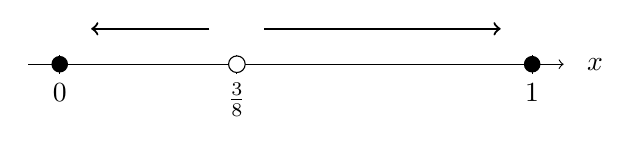
\begin{tikzpicture}[scale=1.0]
\draw[->] (-0.4,0) -- (6.4,0);
\foreach \x/\lab in {0/$0$, 2.25/$\frac{3}{8}$, 6/$1$} { \draw (\x,0.12)--(\x,-0.12) node[below] {\lab}; }
\fill (0,0) circle (3pt);
\draw[fill=white] (2.25,0) circle (3pt);
\fill (6,0) circle (3pt);
\draw[->,thick] (1.9,0.45) -- (0.4,0.45);
\draw[->,thick] (2.6,0.45) -- (5.6,0.45);
\node at (6.8,0) {$x$};
\end{tikzpicture}
\end{center}
So both $x=0$ and $x=1$ are asymptotically stable and $x^*=\frac{3}{8}$ is unstable. The system is bistable, and $x^*$ separates the two basins of attraction: $\left[ 0,\frac{3}{8} \right)$ leads to all D and $\left( \frac{3}{8},1 \right]$ leads to all C.

For a population stuck in the all-D state, $x^*=\frac{3}{8}$ is the critical mass. Converting a few individuals achieves nothing, because they are below the threshold and the dynamics push them back down. Converting more than $\frac{3}{8}$ of the population at once, however, tips the system, and the rest follows by itself.

\item Here $a=-1$, $b=2$, $c=0$, $d=1$, so $a-c=-1$ and $b-d=1$:
\[ \frac{\dd x}{\dd t} = x(1-x)\left[ -x+(1-x) \right] = x(1-x)(1-2x) . \]
The equilibria are $x=0$, $x=1$, and $x^*=\frac{1}{2}$. The bracket is positive for $x<\frac{1}{2}$ and negative for $x>\frac{1}{2}$, so the flow points toward $x^*$ from both sides:
\begin{center}
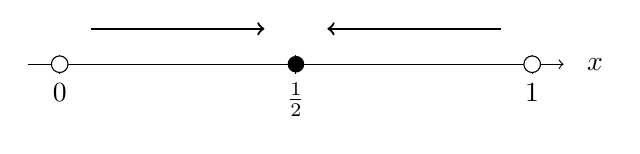
\begin{tikzpicture}[scale=1.0]
\draw[->] (-0.4,0) -- (6.4,0);
\foreach \x/\lab in {0/$0$, 3/$\frac{1}{2}$, 6/$1$} { \draw (\x,0.12)--(\x,-0.12) node[below] {\lab}; }
\draw[fill=white] (0,0) circle (3pt);
\fill (3,0) circle (3pt);
\draw[fill=white] (6,0) circle (3pt);
\draw[->,thick] (0.4,0.45) -- (2.6,0.45);
\draw[->,thick] (5.6,0.45) -- (3.4,0.45);
\node at (6.8,0) {$x$};
\end{tikzpicture}
\end{center}
Equivalently, differentiating the right-hand side $g(x) = x(1-x)(1-2x) = x-3x^2+2x^3$ gives $g'(x)=1-6x+6x^2$, and $g'\!\left( \frac{1}{2} \right) = 1-3+\frac{3}{2} = -\frac{1}{2}<0$, confirming that $x^*=\frac{1}{2}$ is asymptotically stable. Both pure states are unstable.

Neither pure strategy is Nash here, as Problem 7(d) implied, and the population settles instead at the mixture in which half of the contests are escalated.

\end{enumerate}

\subsection*{Solution to Problem 9}

\begin{enumerate}[label=(\alph*)]
\item The first round is always played. Round $n$ is played if the game has continued $n-1$ times, which happens with probability $w^{n-1}$. Hence the expected number of rounds is
\[ \sum_{n=1}^{\infty} w^{n-1} = \frac{1}{1-w} , \]
which converges because $0<w<1$.

\item The largest conceivable expected score is obtained by collecting the largest entry of the matrix, $T=5$, in every round, which requires an opponent who cooperates in every round no matter what. So a player meeting ALLC and defecting throughout gets
\[ \frac{T}{1-w} = \frac{5}{1-w} . \]

\item Write $m = \frac{1}{1-w}$ for the expected number of rounds.
\begin{itemize}
\item TFT versus TFT: both cooperate in round $1$; each then sees a C and cooperates again, and so on forever. Both get $R$ in every round:
\[ u(\text{TFT},\text{TFT}) = \frac{R}{1-w} = \frac{3}{1-w} . \]
\item TFT versus ALLD: in round $1$, TFT plays C and ALLD plays D, so TFT gets $S=0$ and ALLD gets $T=5$. From round $2$ on, TFT retaliates and both defect, each getting $P=1$. The expected number of rounds after the first is $m-1=\frac{w}{1-w}$, so
\[ u(\text{TFT},\text{ALLD}) = 0 + \frac{w}{1-w}, \qquad
u(\text{ALLD},\text{TFT}) = 5 + \frac{w}{1-w} = \frac{5-4w}{1-w} . \]
\item TFT versus ALLC: both cooperate in every round (TFT is never provoked), so both get $\frac{3}{1-w}$, the same as TFT versus TFT.
\item ALLD versus ALLC: ALLD gets $T$ and ALLC gets $S$ in every round:
\[ u(\text{ALLD},\text{ALLC}) = \frac{5}{1-w}, \qquad u(\text{ALLC},\text{ALLD}) = 0 . \]
\item ALLD versus ALLD: both get $P$ in every round, $\frac{1}{1-w}$ each.
\end{itemize}
Already visible here is the point of the repeated game: $\frac{3}{1-w}$, earned by two reciprocators, beats the $\frac{1}{1-w}$ that two defectors earn, so there is something to be gained from cooperating if it can be protected.

\item A rare mutant meets residents almost always, so we compare the payoffs against a TFT opponent. TFT resists ALLD if and only if
\[ u(\text{TFT},\text{TFT}) > u(\text{ALLD},\text{TFT}),
\qquad\text{that is,}\qquad
\frac{R}{1-w} > T + \frac{wP}{1-w} . \]
Multiplying by $1-w>0$,
\[ \begin{aligned}
R &> T(1-w)+wP = T - w\left( T-P \right)\\
&\Longrightarrow\quad w\left( T-P \right) > T-R
\quad\Longrightarrow\quad
w > \frac{T-R}{T-P} ,
\end{aligned} \]
where $T-P>0$ makes the last division legitimate. With our numbers,
\[ w > \frac{5-3}{5-1} = \frac{1}{2} . \]
In words: defecting against a reciprocator buys a one-time windfall of $T-R=2$ and then costs $R-P=2$ in every later round. The relationship has to be likely enough to continue for those later losses to outweigh the windfall, and here that means the probability of meeting again must exceed $\frac{1}{2}$. Reciprocity pays only in the shadow of a sufficiently long future.

\item From (b),
\[ u(\text{TFT},\text{TFT}) = u(\text{ALLC},\text{TFT})
= u(\text{TFT},\text{ALLC}) = u(\text{ALLC},\text{ALLC}) = \frac{3}{1-w} . \]
The ESS conditions of Problem 7 with $x=\text{TFT}$ and $y=\text{ALLC}$ then read: condition (i) holds but only with equality, so we must check condition (ii), which demands $u(\text{TFT},\text{ALLC})>u(\text{ALLC},\text{ALLC})$. The two are equal, so condition (ii) fails. Hence TFT is not an ESS, for any value of $w$. The reason is simple: against opponents who never defect, TFT and ALLC are indistinguishable, because TFT's retaliation is never triggered.

What then happens over a long time is the classical story. ALLC mutants are not selected against, so they accumulate in the population by random drift, and the population slowly becomes a mixture of TFT and ALLC that still looks perfectly cooperative. But once the ALLC players are numerous enough, an ALLD mutant does well: it exploits every ALLC it meets and loses only against the TFT players. Cooperation then collapses, until TFT (or something like it) invades the defectors again. Evolutionary simulations of the repeated prisoner's dilemma indeed show exactly these cycles.

\end{enumerate}

\end{document}
